%%%%%%%%%%%%%%%%%%%%%%%%%%%%%%%%%%%
% SCOPO DEL DOCUMENTO
%%%%%%%%%%%%%%%%%%%%%%%%%%%%%%%%%%%
\section{Introduzione}
\subsection{Scopo del documento}\label{sec:scopo_del_documento}
    Lo scopo del seguente documento è quello di illustrare le funzionalità fornite dall'applicazione e fornire agli utenti le istruzioni necessarie per il corretto utilizzo 
    della stessa. Si intende inoltre informare ogni utente sui requisiti minimi necessari per la corretta esecuzione dell'applicativo, al fine di offrire un'esperienza utente chiara ed esaustiva.

%%%%%%%%%%%%%%%%%%%%%%%%%%%%%%%%%%%
% SCOPO DEL PROGETTO
%%%%%%%%%%%%%%%%%%%%%%%%%%%%%%%%%%%
\subsection{Scopo del prodotto}\label{sec:scopo_del_progetto}
    Il prodotto nasce nell'ambito dei \textbf{sistemi gestionali di magazzino}, noti come \textit{Warehouse Management Systems}\textsuperscript{G} (WMS), con l'obiettivo di risolvere una serie di problematiche derivanti dalle soluzioni tradizionali ancora presenti sul mercato. 
    
    Il focus principale è migliorare l'esperienza utente attraverso la realizzazione di un'applicazione che offra un'interazione con il magazzino in un ambiente di lavoro 3D. 
    
    Questo approccio innovativo rispetto ai sistemi tradizionali in 2D permetterebbe una comprensione più approfondita degli spazi, offrendo una visualizzazione intuitiva e completa del magazzino. Ciò consentirebbe agli utenti di prendere decisioni più efficaci ed efficienti, ottimizzando i processi logistici.

    Per raggiungere questo obiettivo, l'ambiente di lavoro non si limita a una semplice visualizzazione del magazzino. Infatti, gli utenti devono poter:
    \begin{itemize}
        \item Spostarsi all'interno dell'ambiente 3D;
        \item Progettare le scaffalature che sono presenti nel magazzino e modificarle nel tempo;
        \item Simulare i flussi di movimento di prodotti.
    \end{itemize}

    Il prodotto si concretizza dunque in una web app, pensata per essere facilmente accessibile agli impiegati d'ufficio, e offre una varietà di funzionalità, tra cui la visualizzazione tridimensionale del magazzino, al fine di migliorare l'esperienza utente.

\subsection{Glossario}
Al fine di evitare ambiguità nei termini utilizzati all’interno del documento, nella sezione \ref{sec:glossario} è presente il ``Glossario'',  in cui sono definiti tutti i termini con specifiche definizioni. Nel testo, un termine presente nel Glossario è identificato in corsivo con una ’G’ in apice.
\newpage


%%%%%%%%%%%%%%%%%%%%%%%%%%%%%%%%%%%
% REQUISITI E COMPATIBILITA'
%%%%%%%%%%%%%%%%%%%%%%%%%%%%%%%%%%%
\section{Requisiti e compatibilità}\label{sec:requisiti_e_compatibilità}
    In questa sezione sono illustrati i requisiti minimi necessari per una corretta esecuzione dell'applicativo realizzato. Saranno quindi evidenziate le caratteristiche 
    che ogni terminale deve soddisfare per configurare correttamente l'ambiente di esecuzione.

    \subsection{Requisiti software}\label{sec:requisiti_e_compatibilità:software}
    L'applicativo sarà reso disponibile all'utente attraverso due modalità: la \textit{modalità utente}\textsuperscript{G} e la \textit{modalità programmatore}\textsuperscript{G}.
    A seconda della modalità selezionata, saranno necessari requisiti software distinti.

    \bigskip
    \noindent Per la \textit{modalità programmatore} saranno necessari: 
    \begin{itemize}
        \item l'installazione del software Node.js, alla versione 20.0 o superiore;
        \item un browser stabile. 
    \end{itemize}
    Per una corretta installazione del software Node.js si rimanda alla pagina dedicata, presente nella sezione \hyperref[sec:riferimenti_esterni]{Riferimenti Esterni} del documento. 
    Per quanto riguarda i browser, l'applicativo è stato testato per il corretto funzionamento con i principali motori di ricerca, che si riportano qui sotto.
    \renewcommand{\arraystretch}{1.5}
    \begin{xltabular}{\textwidth}{ X | X}

        \rowcolor{black}
        \textbf{\color{white} Motore di ricerca} & \textbf{\color{white} Versione}\\ 
        \hline
        \endhead

        Google Chrome & 124.0 \\
        \hline

        Microsoft Edge & 124.0 \\
        \hline
        
        Safari & 17.0 \\
        \hline

        Mozilla Firefox & 115.0 \\
        \hline

        Opera & 109.0 \\
        \hline
        
        \caption{Tabella dei requisiti software - Compatibilità dei browser}
        \label{tab:requisiti:soft}
    \end{xltabular}
    \noindent La \textit{modalità utente} è invece accessibile anche da utenti meno esperti. Non necessita, infatti, di particolari configurazioni e software. Tuttavia, si raccomanda 
    comunque di utilizzare uno dei browser sopra citati. \\



    \subsection{Requisiti hardware}\label{sec:requisiti_e_compatibilità:hardware}
    L'applicativo realizzato appartiene alla categoria delle web-app. Come tale, non sono dunque richiesti dei particolari requisiti hardware per l'esecuzione.
    
    Viene comunque consigliato l'utilizzo di un terminale aggiornato che, a titolo di riferimento, può essere identificato in:
    \begin{xltabular}{\textwidth}{ X | X}

        \rowcolor{black}
        \textbf{\color{white} Componente} & \textbf{\color{white} Requisito minimo consigliato}\\ 
        \hline
        \endhead
        
        Connessione Internet & Connessione Internet stabile e veloce \\
        \hline

        Processore & Quad-Core 1,80 GHz \\
        \hline
        
        Memoria RAM & 8GB DDR3 \\
        \hline

        \caption{Tabella dei requisiti hardware}
        \label{tab:requisiti:hard}
    \end{xltabular}

    \newpage

    

%%%%%%%%%%%%%%%%%%%%%%%%%%%%%%%%%%%
% INSTALLAZIONE ED ESECUZIONE
%%%%%%%%%%%%%%%%%%%%%%%%%%%%%%%%%%%
\section{Installazione ed esecuzione}\label{sec:install_run}
    L'esecuzione dell'applicazione differisce in base alla modalità di esecuzione scelta. Pertanto si riportano separatamente le due modalità disponibili. 

    \subsection{Modalità programmatore}\label{sec:install_run:esperto}
    Questa sezione intende definire le operazioni di installazione preliminari necessarie per l'esecuzione dell'applicativo in \textit{modalità programmatore}.\\ 
    Di seguito saranno quindi elencati i passaggi necessari per la clonazione del repository\textsuperscript{G} e l'avvio dell'applicazione. \\
    Si consiglia di optare per questa modalità solo se si è esperti nell'uso dei software.
    
    \subsubsection{Clonazione del repository}\label{sec:install_run:esperto:clone}
    Per scaricare tutti i file necessari all'esecuzione è possibile: 
    \begin{enumerate}
        \item Scaricare il codice (archivio in formato \textit{.zip}) direttamente dal seguente link: \\  
        \url{https://github.com/Avant-Garde-Software-Engineering/WMS3D.git} \textcolor{gray}{\textit{(ultimo accesso 08-05-24)}}
        \item Clonare il repository utilizzando i servizi messi a disposizione dal software Git, che deve però essere precedentemente installato sulla macchina di esecuzione:
        \begin{itemize}
            \item Posizionarsi sul repository locale di interesse;
            \item Utilizzare il comando:\\
            \textbf{git clone \url{https://github.com/Avant-Garde-Software-Engineering/WMS3D.git}}.
        \end{itemize}
    \end{enumerate}

    \subsubsection{Avvio dell'applicativo}\label{sec:install_run:esperto:avvio}
    Dopo aver creato una copia del codice nel repository locale, ci si deve posizionare all'interno della sotto-cartella \textbf{src}. \\
    Successivamente, sarà quindi necessario aprire un terminale in tale directory ed eseguire i seguenti passaggi:
    \begin{enumerate}
        \item Installare le dipendenze del progetto con il comando (necessario solamente al primo avvio): \\
        \textbf{npm install}
        \item Compilare l'applicazione con il comando: \\  
        \textbf{npm run dev}
        \item Una volta terminata la fase di build dell'applicativo, aprire un browser e ricercare la seguente pagina web per visualizzare la web-app: \\  
        \url{http://localhost:3000}
    \end{enumerate}

    \subsection{Modalità utente}\label{sec:install_run:user}
    Come accennato, la \textit{modalità utente} non necessita di alcuna procedura preliminare. L'utente dovrà solamente collegarsi al seguente link per poter eseguire direttamente la web-app dal proprio browser predefinito: 
    \begin{center}
        \url{https://wms-3-d-src.vercel.app/} \\ \textcolor{gray}{\textit{(ultimo accesso 08-05-24)}}
    \end{center}

    \newpage



    
%%%%%%%%%%%%%%%%%%%%%%%%%%%%%%%%%%%
% ISTRUZIONI D'USO 
%%%%%%%%%%%%%%%%%%%%%%%%%%%%%%%%%%%
\section{Istruzioni d'uso}\label{sec:Istruzioni_uso}

    \subsection{Configurazione del magazzino}\label{sec:creazione}
        Nell'applicativo realizzato non è necessaria alcuna login iniziale. L'applicativo si presenta quindi subito con la schermata iniziale in cui l'utente è 
        invitato ad inserire tutti i dati necessari per poter configurare o caricare il magazzino da visualizzare.
        \begin{figure}[h!]
            \centering
            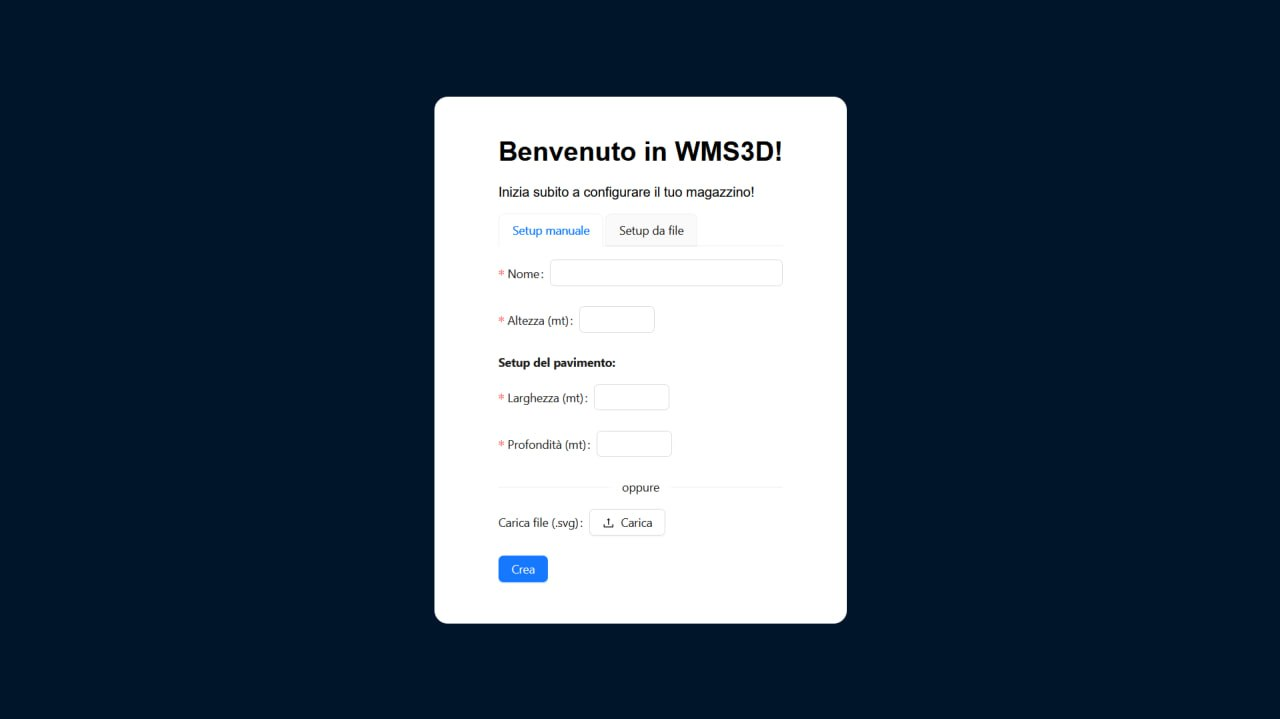
\includegraphics[width=0.9\textwidth]{images/schermata_iniziale.png}
            \caption{Configurazione del magazzino - Setup manuale}
        \end{figure}\\
        \noindent In questa sezione l'utente potrà scegliere se configurare manualmente il magazzino (\textit{Setup manuale}) o, in alternativa, caricare un layout già pronto all'uso (\textit{Setup da file}).
        
        \subsubsection{Configurazione manuale del magazzino}\label{sec:creazione:configurazione}
            Se la scelta ricade sulla configurazione manuale del magazzino l'utente dovrà inserire nell'apposito form i seguenti dati: 
            \begin{itemize}
                \item Un \textbf{nome} da assegnare al magazzino;
                    \begin{itemize}
                        \item \textit{Formato accettato}: massimo 20 caratteri, scelti tra lettere (sia maiuscole che minuscole), numeri e "\_".
                    \end{itemize}
                \item L'\textbf{altezza} (espressa in metri) del magazzino;
                     \begin{itemize}
                        \item \textit{Formato accettato}: un numero nel range 0.01mt-50mt con una precisione di due cifre decimali.
                    \end{itemize}
                \item La \textbf{pianta del magazzino}, con due opzioni disponibili:
                \begin{enumerate}
                    \item Impostare una semplice pianta rettangolare, andando a indicare le misure di larghezza e profondità (sempre espresse in metri);
                         \begin{itemize}
                            \item \textit{Formato accettato}: un numero nel range 0.01mt-1000mt con una precisione di due cifre decimali.
                        \end{itemize}
                    \item Caricare una pianta personalizzata, andando a caricare un file .svg appositamente realizzato.
                        \begin{itemize}
                            \item \textit{Formato accettato}: file .svg contenente il tag \textit{polygon} con proprietà \textit{points} definita (per almeno 3 punti).
                        \end{itemize}
                \end{enumerate}
            \end{itemize}
            Durante l'inserimento di ciascun campo, sia numerico che testuale, l'utente sarà comunque aiutato dal sistema al fine di inserire correttamente i dati richiesti.\\
            Sarà infatti assistito durante la fase di inserimento degli input in modo tale da garantire una corretta configurazione iniziale del magazzino.

            \paragraph{Caricamento pianta da file .svg} \label{sec:creazione:configurazione:svg}
            Come spiegato in precedenza, l'utente ha la possibilità di caricare una pianta personalizzata attraverso un apposito file .svg.
            
            In caso di caricamento di un file non conforme, che non rispetta il formato sopra citato, sarà visualizzato un messaggio di errore e l'utente potrà rieseguire l'operazione. 
            \begin{figure}[h!]
                \centering
                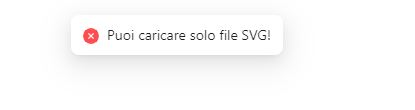
\includegraphics[]{images/errore_caricamento_svg.png}
                \caption{Configurazione magazzino - Errore caricamento .svg (messaggio)}
            \end{figure}

            Tuttavia, è possibile comunque ricevere un altro messaggio di errore nel caso in cui le dimensioni della pianta non rispettino i limiti di larghezza e profondità del magazzino (range compreso tra 0.01 e 1000mt). In tal caso, sarà visualizzato una finestra modale di errore simile alla seguente.
            \begin{figure}[H]
                \centering
                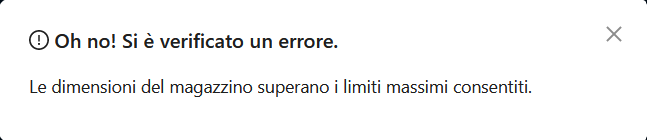
\includegraphics[]{images/svg_error_modal.png}
                \caption{Configurazione magazzino - Errore caricamento .svg (modale)}
            \end{figure}
            \noindent Una volta chiusa questa finestra, l'utente potrà rieseguire l'operazione.
        
        
        \subsubsection{Caricamento del magazzino da file}\label{sec:creazione:caricamento}
            Nel caso in cui l'utente abbia già salvato tramite l'applicazione la configurazione di un magazzino, egli avrà la possibilità di ricaricare quanto già realizzato grazie all'apposita sezione. 
            \begin{figure}[H]
                \centering
                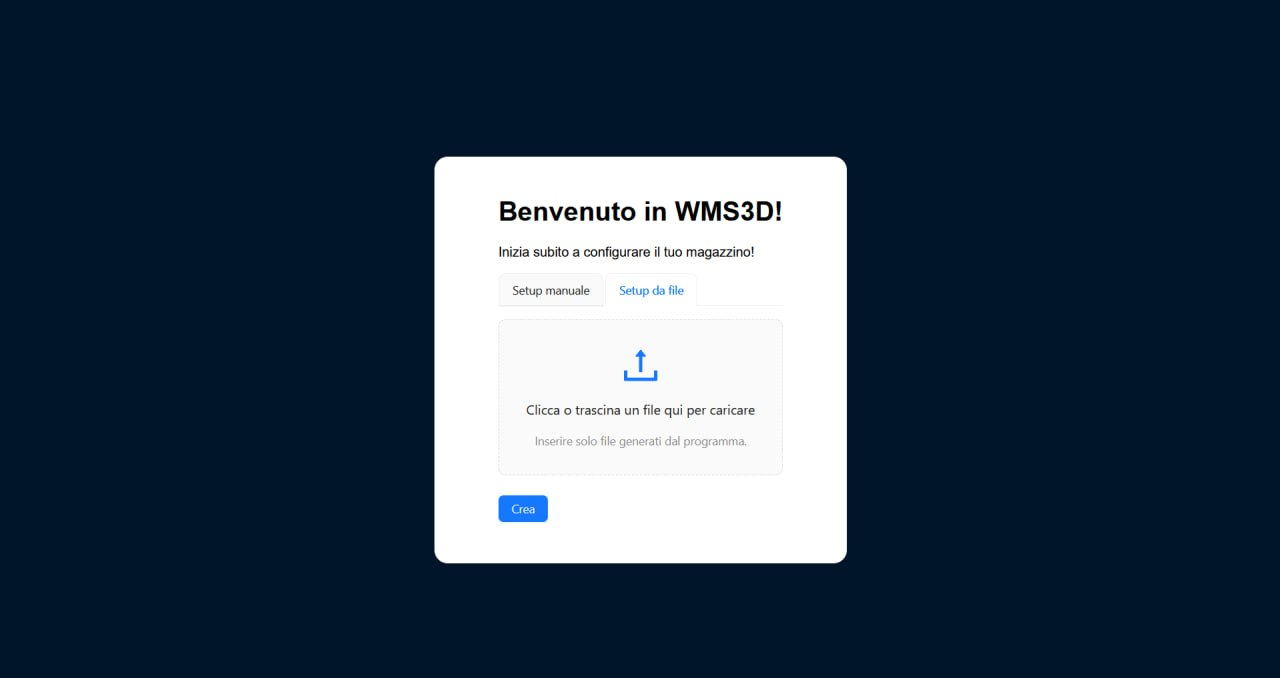
\includegraphics[width=0.9\textwidth]{images/caricamento.png}
                \caption{Configurazione del magazzino - Setup da file}
            \end{figure}
           \noindent In particolare, in questa sezione, è possibile caricare un singolo \textbf{file .json} precedentemente generato dall'applicazione, consentendo così di configurare il magazzino in modo identico alla sessione precedente.
           
           Analogamente al caricamento della pianta da file .svg, anche in questo caso sarà il sistema a verificare la correttezza del tipo di file che si sta cercando di importare mostrando, tramite messaggi e finestre modali, l'errore riscontrato. Tuttavia, si raccomanda vivamente l'uso esclusivo di file generati dall'applicazione e non modificati/creati esternamente. Non si assicura, infatti, il corretto funzionamento dell'applicativo in caso di tali modifiche non autorizzate.
    \newpage        

    \subsection{Warehouse Management System}\label{sec:principale}
        \subsubsection{Interfaccia utente principale}
        Una volta configurato correttamente il magazzino l'utente si troverà di fronte alla pagina principale dell'applicativo. 
        In questa pagina troverà: 
        \begin{itemize}
            \item Una \textbf{barra di navigazione}, composta da due pulsanti: 
            \begin{itemize}
                \item un pulsante usato per nascondere o mostrare la sidebar laterale, posto sull'estrema sinistra;
                \item un pulsante usato per il salvataggio del magazzino, posizionato sull'estrema destra. Attraverso quest'ultimo bottone sarà possibile scaricare il file .json di configurazione del magazzino. Questo file conterrà tutte le informazioni in merito al magazzino stesso, finora creato.
            \end{itemize}
            \item Una sidebar, posta sulla sinistra, che supporta l'utente fornendo una panoramica degli elementi presenti nel magazzino. Questa sezione viene chiamata \textbf{libreria}\textsuperscript{G}. 
            \item La \textbf{sezione 3D} nella quale viene renderizzato il magazzino. In essa troveremo quindi la rappresentazione di uno spazio tridimensionale in cui sono identificabili:
            \begin{itemize}
                \item Una superficie bianca e piana suddivisa in quadrati di uguale dimensione, ciascuno rappresentante un metro quadrato, utilizzata come griglia di riferimento per l'utente.
                \item Una porzione della suddetta superficie evidenziata in giallo, a rappresentare la pianta del magazzino.
                \item Delle superfici grigio chiaro, che si sviluppano a partire dalla porzione di piano evidenziata, che rappresentano i muri del magazzino.
                \item Se presenti, gruppi di blocchi ``cavi'' di colore grigio/nero rappresentanti le scaffalature. Ogni blocco rappresenta un bin\textsuperscript{G} della scaffalatura, e le coordinate sono visibili all'interno di ciascun blocco.
                \item Se presenti, dei cubi posizionati all'interno dei bin (solo uno per bin) a rappresentare dei prodotti posizionati.
            \end{itemize}
        \end{itemize}
        \begin{figure}[h!]
            \centering
            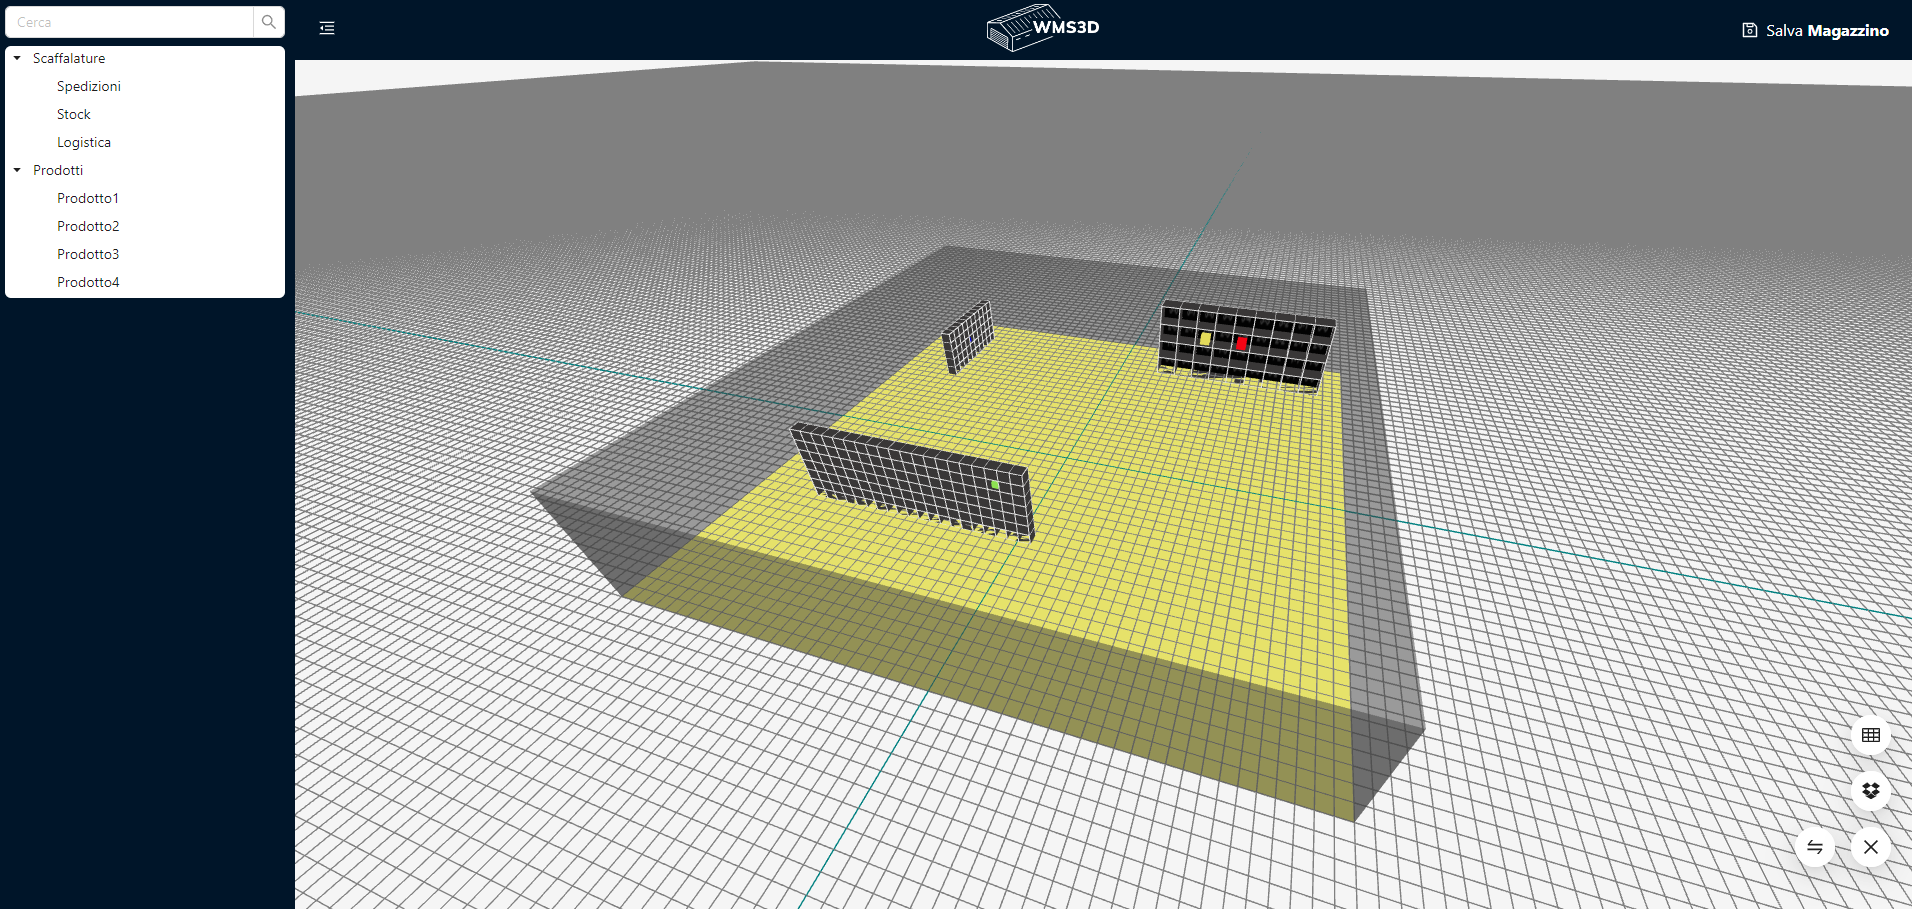
\includegraphics[width=0.9\textwidth]{images/schermata_principale.png}
            \caption{Schermata principale dell'applicativo}
        \end{figure}

        \subsubsection{Esplorazione e ricerca}\label{sec:principale:esplorare}
            \paragraph{Navigazione all'interno del render 3D} \label{sec:principale:esplorare:navigare}
               Per abilitare (o disabilitare) la navigazione all'interno del magazzino è sufficiente cliccare il \textbf{tasto centrale del mouse}. 
               Una volta abilitata, all'interno della sezione 3D, l'utente potrà navigare tramite mouse o tastiera, permettendo così di cambiare la vista del magazzino secondo le proprie preferenze.
               
                In particolare, supponendo un utilizzo da parte di un mouse a tre tasti (il tasto destro, il tasto sinistro e il tasto centrale, o rotella), l'utilizzatore potrà:
                \begin{itemize}
                    \item effettuare uno zoom in/out attraverso il \textbf{tasto centrale};
                    \item cambiare angolazione e prospettiva di visualizzazione attraverso \textbf{tasto destro e sinistro}.
                \end{itemize}
                Da tastiera, invece, sono garantiti i seguenti comandi: 
                \begin{itemize}
                    \item \textbf{Tasto W}: zoom in;
                    \item \textbf{Tasto S}: zoom out;
                    \item \textbf{Tasto D}: spostamento verso destra;
                    \item \textbf{Tasto A}: spostamento verso sinistra.
                \end{itemize}
                L'utente avrà quindi modo di muoversi liberamente all'interno del render 3D, mantenendo però il focus sul magazzino ed il suo contenuto. 

            \paragraph{Selezionare elementi}
               In presenza di scaffalature posizionate, l'utente sarà in grado di selezionare le scaffalature stesse o singoli bin dal render 3D semplicemente cliccando su di essi (per il bin solo dopo aver selezionato prima la scaffalatura). 
               Una volta selezionato un componente comparirà una Card\textsuperscript{G}, in alto a destra, in grado di fornire le informazioni sull'oggetto selezionato e, 
                in aggiunta, verrà rimarcato il componente selezionato anche all'interno della libreria. 

                 Analogamente, è possibile selezionare una scaffalatura o un prodotto\textsuperscript{G} (ma non un singolo bin) dalla libreria. Anche in questo caso, si aprirà la Card corrispondente e verrà rimarcato il componente selezionato anche all'interno del render 3D (nel caso di prodotti, solo se effettivamente posizionati in bin). 

                \bigskip
                \noindent Dal render 3D la selezione sarà evidenziata nel seguente modo:
                \begin{itemize}
                    \item \textbf{Selezione di scaffalatura:} la scaffalatura sarà evidenziata in verde;
                    \item \textbf{Selezione di bin:} il bin sarà evidenziato in verde e gli spigoli del prodotto in esso contenuto (se presente) saranno evidenziati in arancione; 
                    \item \textbf{Selezione di prodotto:} gli spigoli di tutte le copie del prodotto (se presenti) saranno evidenziati in arancione. 
                \end{itemize}

                \noindent Si riportano di seguito, nel dettaglio, le informazioni visualizzate nella Card per ogni tipo di selezione effettuata.

                \subparagraph{Card della scaffalatura.}
                Come accennato, in caso di selezione di una scaffalatura, verranno quindi visualizzate le caratteristiche della scaffalatura stessa nella Card.  \\
                In particolare vengono visualizzate:
                \begin{itemize}
                    \item Nome;
                    \item Capacità della scaffalatura, nel formato [\# bin larghezza]x[\# bin altezza];
                    \item Dimensione dei bin, nel formato [mt in larghezza]x[mt in altezza]x[mt in profondità]).
                \end{itemize}
                \begin{figure}[H]
                    \centering
                    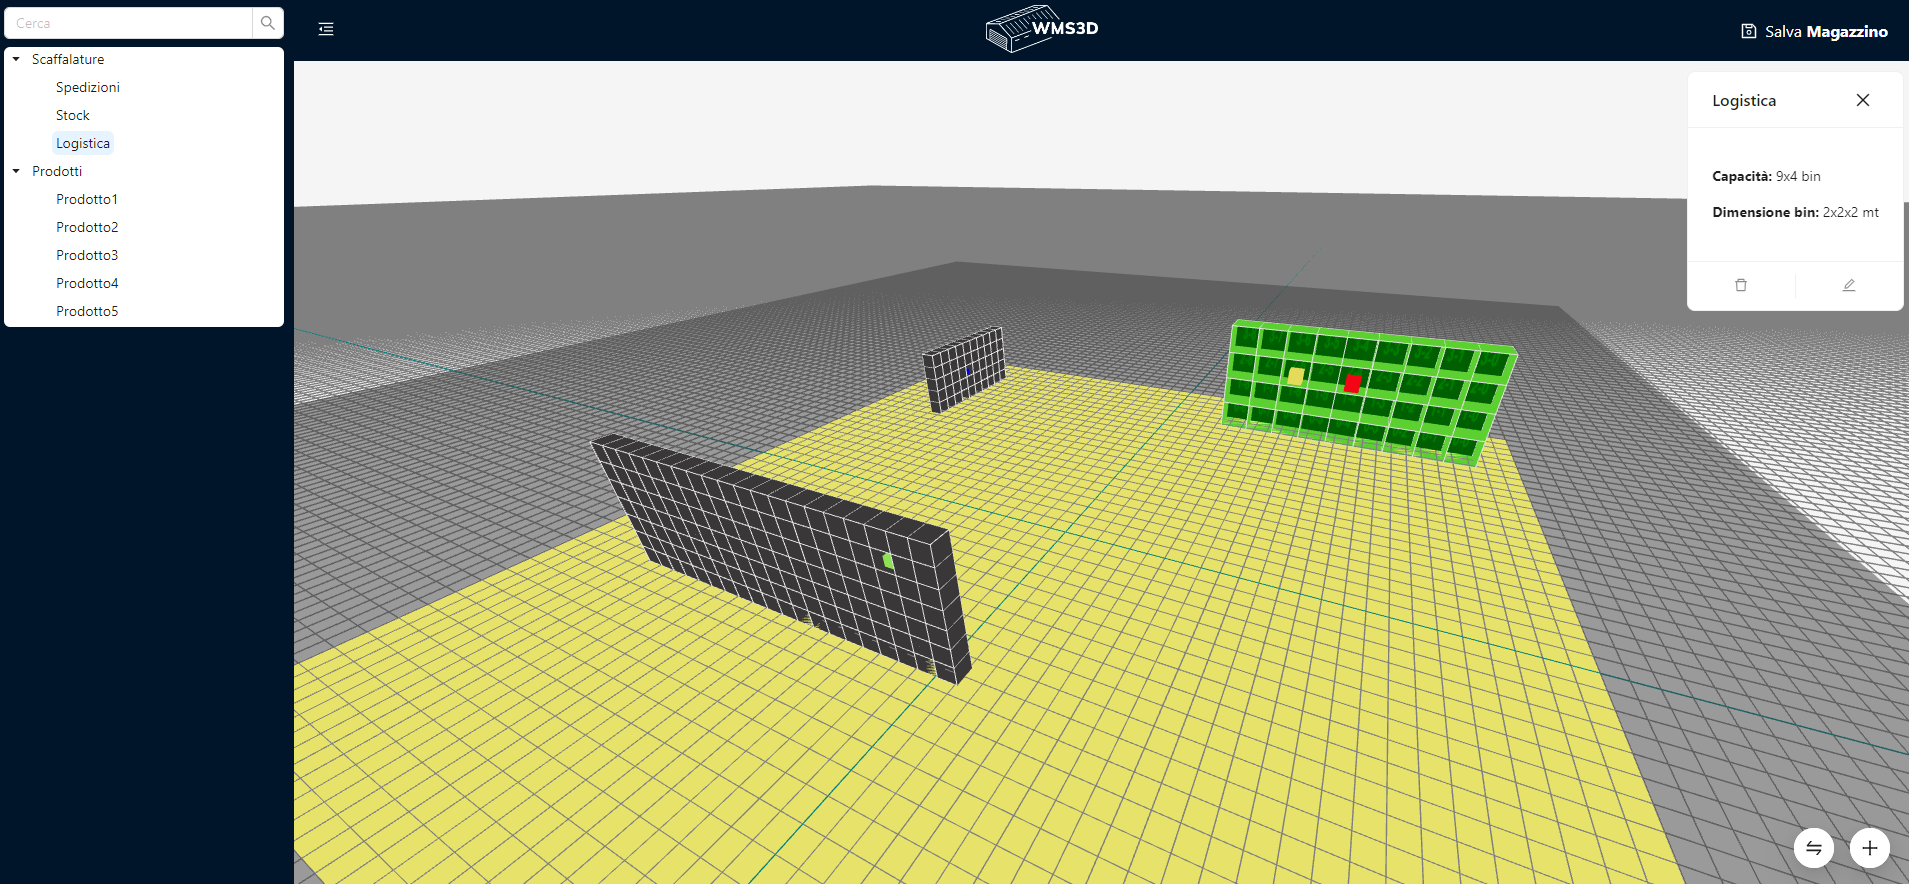
\includegraphics[width=0.9\textwidth]{images/selezione_scaffalatura.png}
                    \caption{Selezione scaffalatura da render 3D o libreria}
                \end{figure}

                \subparagraph{Card del bin.}
                In caso di selezione di uno specifico bin verranno invece visualizzate in una Card le seguenti informazioni:
                \begin{itemize}
                    \item Un codice univoco del bin;
                    \item Lo stato del bin, che può essere: 
                    \begin{enumerate}
                        \item \textbf{Empty}: bin vuoto,
                        \item \textbf{Still}: bin occupato da un prodotto,
                        \item \textbf{Outgoing}: bin occupato da un prodotto per il quale è stata richiesta la movimentazione,
                        \item \textbf{Ingoing}: bin non disponibile per l'inserimento di prodotti, anche se vuoto, in quanto destinazione di una movimentazione pendente;
                    \end{enumerate}
                    \item Il nome del prodotto eventualmente presente nel bin.
                \end{itemize}
                \begin{figure}[h!]
                    \centering
                    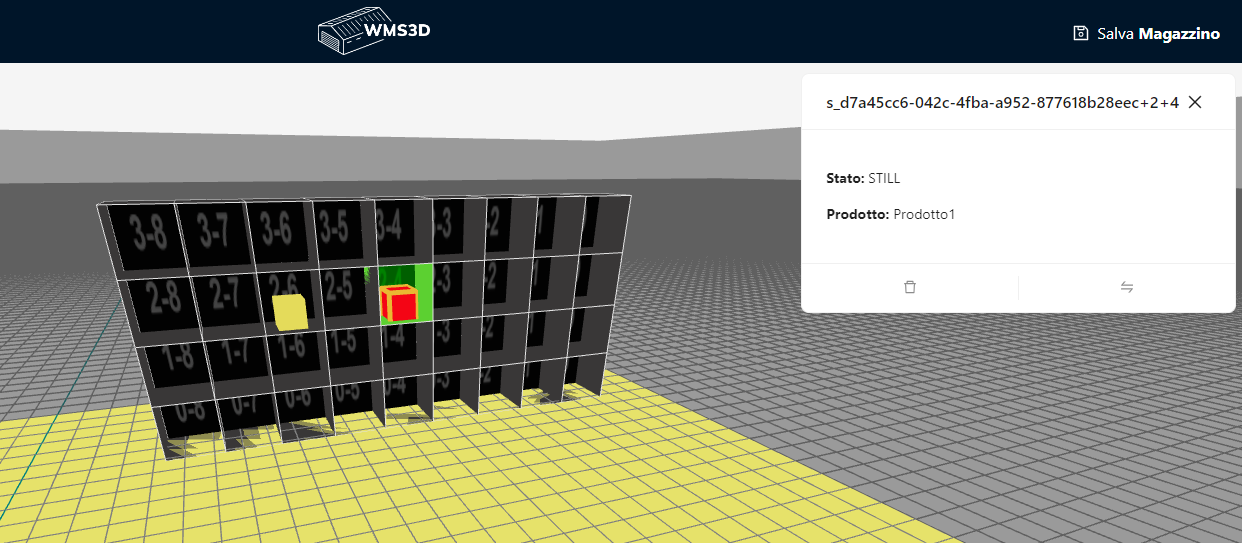
\includegraphics[width=0.9\textwidth]{images/selezione_bin.png}
                    \label{sel_bin}
                    \caption{Selezione bin da render 3D (o da Card del prodotto)}
                \end{figure}

                \subparagraph{Card del prodotto.}
                 In caso di selezione di un prodotto verranno invece visualizzate in una Card le seguenti informazioni:
                \begin{itemize}
                    \item Il nome del prodotto;
                    \item Una lista che mostra tutte le copie del prodotto allocate all'interno del magazzino. Ogni copia è identificata da una coppia scaffalatura-bin, e cliccando su di esse si apre la Card del bin corrispondente.
                \end{itemize}
                \begin{figure}[H]
                    \centering
                    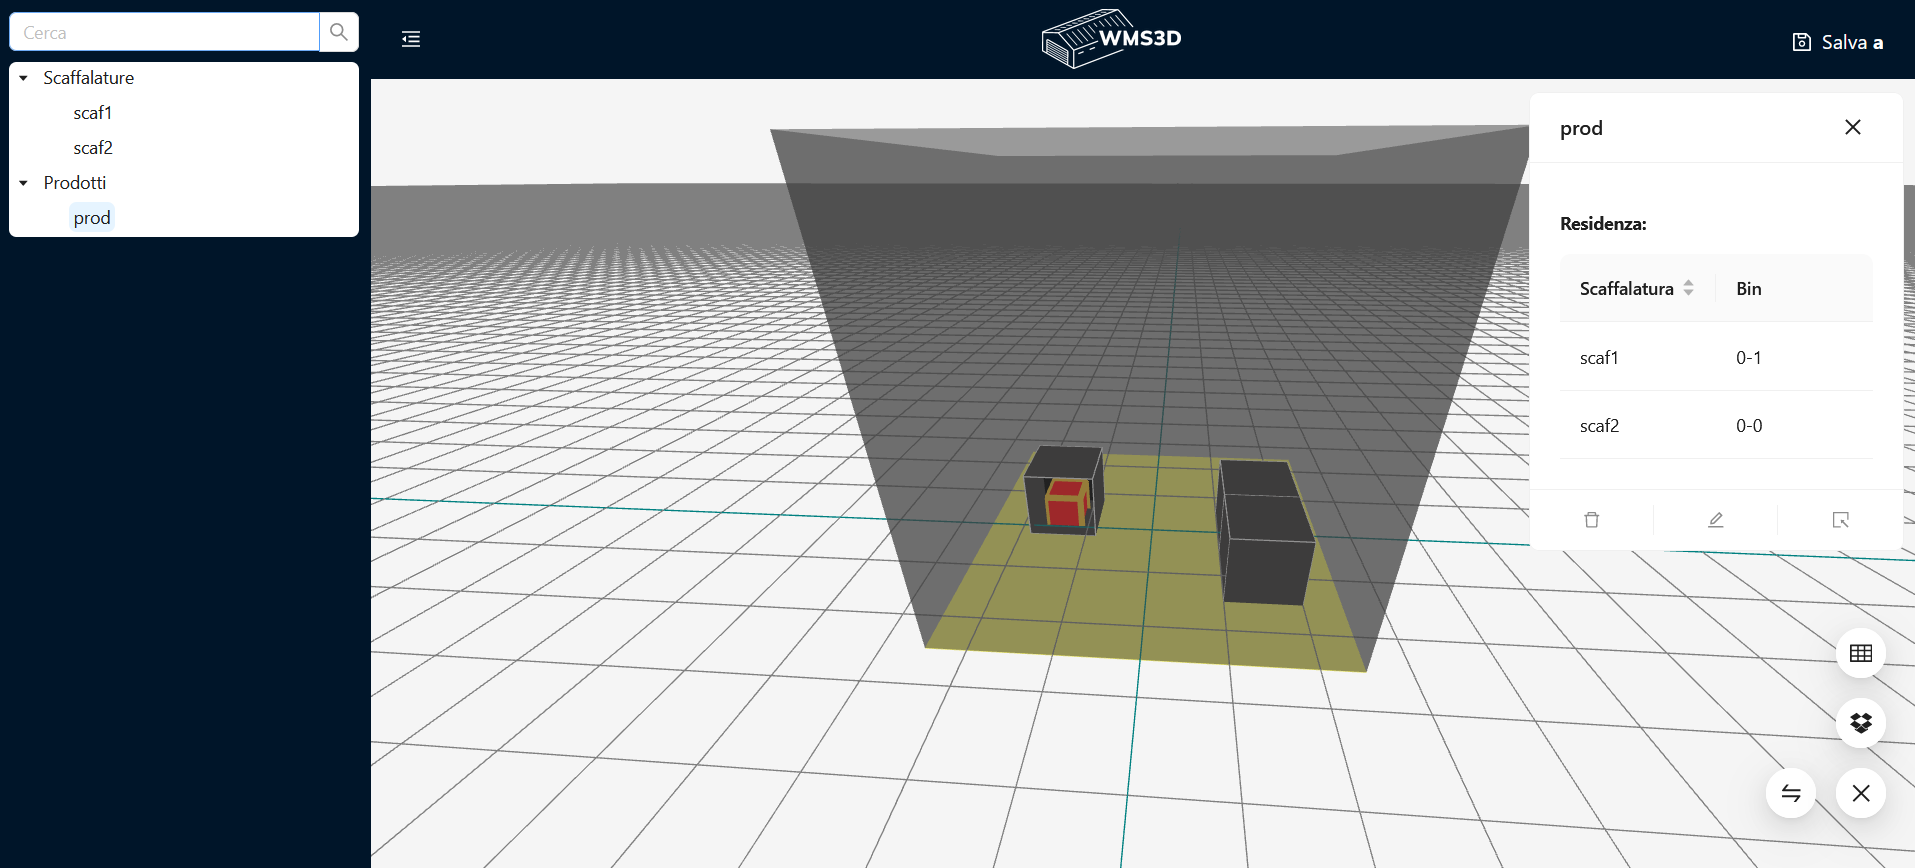
\includegraphics[width=0.9\textwidth]{images/selezione_prodotto_card.png}
                    \label{sel_prod}
                    \caption{Selezione prodotto da libreria}
                \end{figure}

            \subsubsection{Ricercare elementi} \label{sec:principale:esplorare:ricerca}
                Come accennato, all'interno della libreria, sarà possibile visualizzare l'elenco di tutti i componenti finora creati.
                Verranno quindi elencate tutte le scaffalature posizionate all'interno del render e tutti i prodotti creati. Si segnala che \textbf{un prodotto può essere creato
                e non posizionato}. In tal caso sarà quindi elencato in libreria ma non sarà presente sul render 3D.\\
                \begin{figure}[H]
                    \centering
                    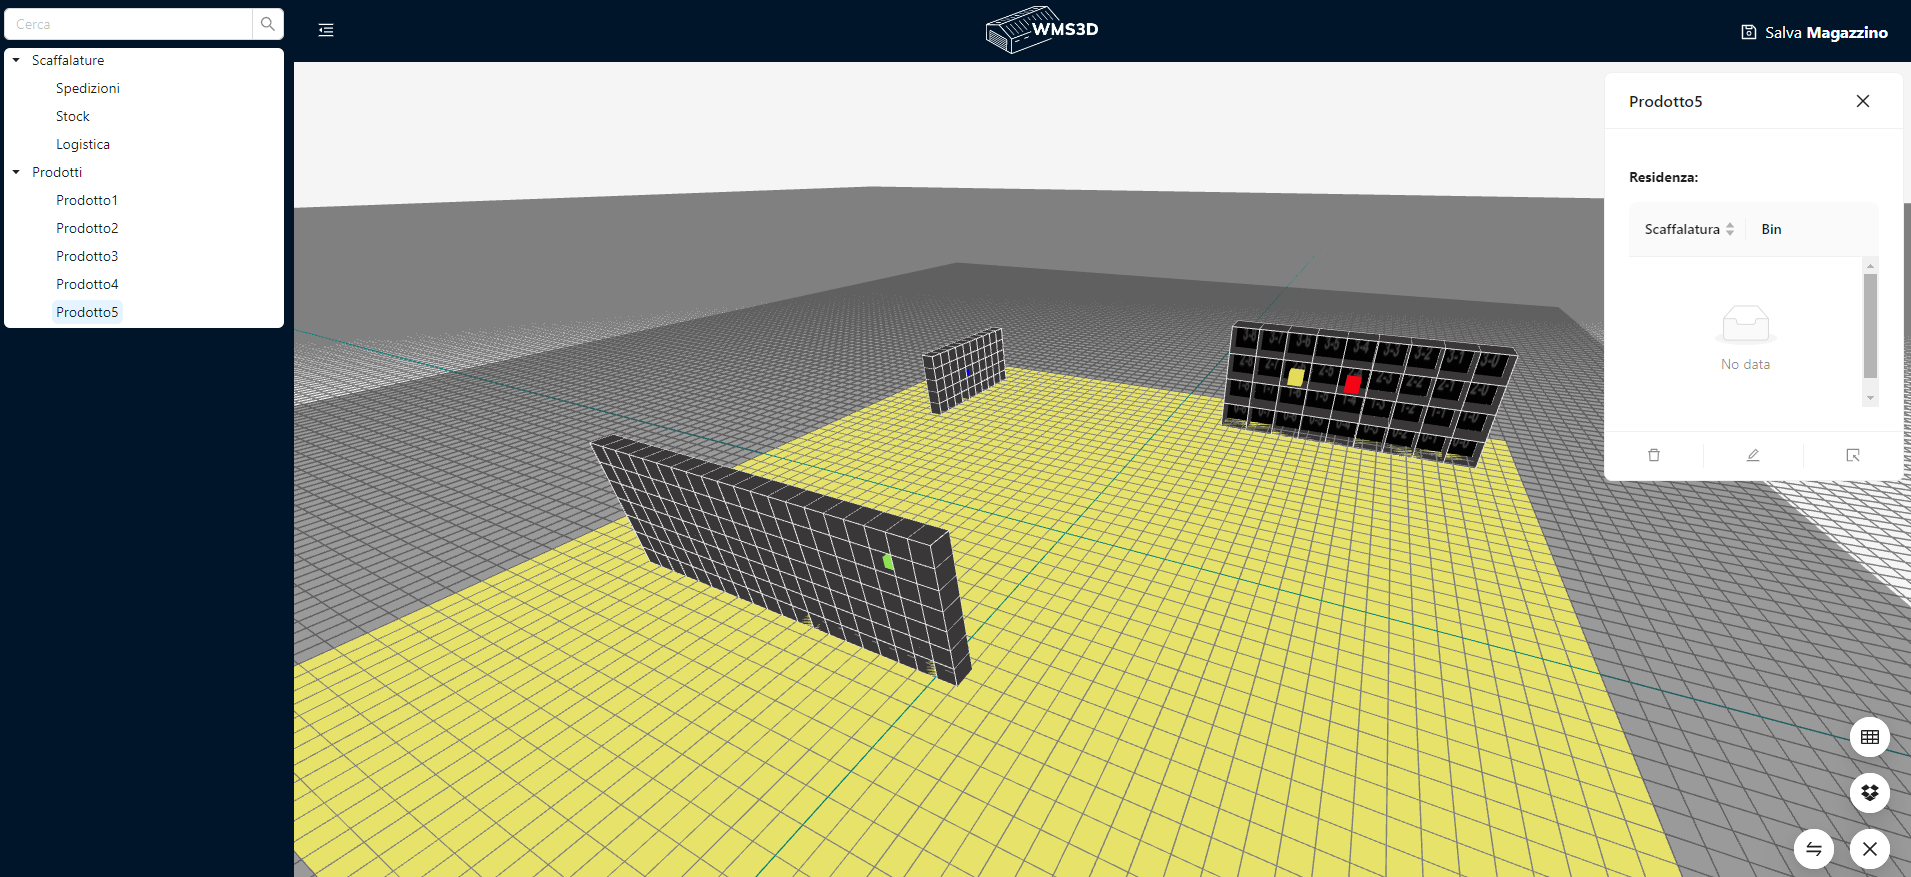
\includegraphics[width=1.0\textwidth]{images/prodotto_no_render.png}
                    \caption{Prodotto aggiunto alla libreria ma non presente sul render}
                \end{figure}
                
                \noindent All'interno della libreria è inoltre presente uno strumento per facilitare la ricerca di uno specifico componente. L'utente, inserendo nell'apposito
                form il nome del componente desiderato, andrà a filtrare il contenuto della libreria per identificare il prodotto/scaffalatura di interesse. \\\
                \begin{figure}[h!]
                    \centering
                    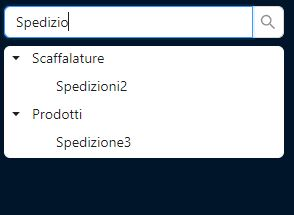
\includegraphics[width=0.4\textwidth]{images/filtro_ricerca.png}
                    \caption{Ricerca da libreria}
                \end{figure}
                
                \noindent Si noti che tutti i componenti presenti in libreria sono ovviamente selezionabili anche in presenza del filtro sopra illustrato.    

    \newpage
    \subsection{Scaffalature}\label{sec:scaffalature}
    In questa sezione si riportano tutte le funzionalità disponibili per gestire le scaffalature del magazzino.
        \subsubsection{Aggiunta scaffalatura}\label{sec:scaffalature:aggiunta}
            Per poter aggiungere una nuova scaffalatura è necessario premere il tasto "+" presente nell'angolo in basso a destra del render 3D.\\
            \begin{figure}[h!]
                \centering
                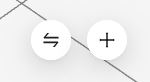
\includegraphics[width=0.3\textwidth]{images/aggiunta_spostamenti.png}
                \caption{Pulsante aggiunta componenti}
            \end{figure}

            \noindent Successivamente, per proseguire, cliccare il tasto relativo all'aggiunta scaffalatura.\\
            \begin{figure}[h!]
                \centering
                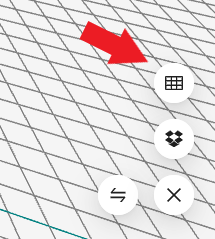
\includegraphics[width=0.3\textwidth]{images/aggiunta_scaffalatura.png}
                \caption{Pulsante aggiunta scaffalatura}
            \end{figure}
            \\
            \noindent Sarà quindi richiesto all'utente di creare la scaffalatura impostando i seguenti campi:
            \begin{itemize}
                \item Il \textbf{nome} che si intende dare alla scaffalatura, attributo univoco della scaffalatura;
                    \begin{itemize}
                        \item \textit{Formato accettato}: massimo 20 caratteri, scelti tra lettere (sia maiuscole che minuscole), numeri e "\_".
                    \end{itemize}
                \item \textbf{Dimensione dei singoli bin}, espressa in metri;
                    \begin{itemize}
                        \item \textit{Formato accettato}: un numero strettamente maggiore di 0.00 con una precisione di due cifre decimali. Tale numero non deve comunque superare l'altezza del magazzino, precedentemente inserita al momento della configurazione dello stesso.
                    \end{itemize}
                \item \textbf{Altezza} della scaffalatura, espressa in numero di bin;
                    \begin{itemize}
                        \item \textit{Formato accettato}: un numero strettamente maggiore di 0.00 con una precisione di due cifre decimali. Tale numero moltiplicato per la dimensione del bin non deve comunque superare l'altezza del magazzino, precedentemente inserita al momento della configurazione dello stesso.
                    \end{itemize}
                \item \textbf{Larghezza} della scaffalatura, espressa in numero di bin.
                    \begin{itemize}
                        \item \textit{Formato accettato}: un numero strettamente maggiore di 0.00 con una precisione di due cifre decimali.
                    \end{itemize}
            \end{itemize}
            \begin{figure}[H]
                \centering
                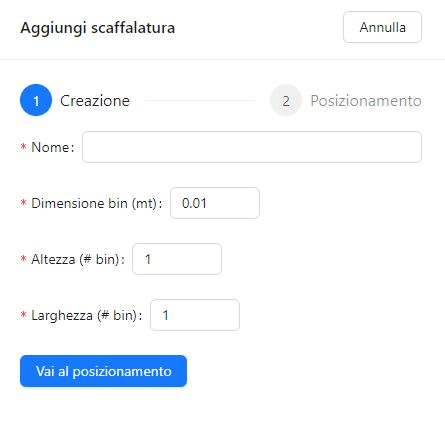
\includegraphics[width=0.4\textwidth]{images/creazione_scaffalatura.png}
                \caption{Form di aggiunta scaffalatura}
            \end{figure}

            \noindent Il passaggio successivo, che completa la creazione, consiste nel posizionare la scaffalatura in uno spazio idoneo del magazzino, in modo tale che non collida con altri elementi presenti nel render e che non oltrepassi i limiti rappresentati dai muri perimetrali.
            
            \subsubsection{Posizionamento scaffalatura}\label{sec:scaffalature:posizionamento}
            Per riuscire a spostare la scaffalatura sarà necessario utilizzare ``l'assistente'' al movimento posto al centro della scaffalatura creata nel render 3D. 
            Sarà infatti presente una traccia per ogni spostamento possibile: 
            \begin{itemize}
                \item spostamento laterale (linea rossa); 
                \item spostamento in profondità (linea blu);
                \item rotazione (linea verde).
            \end{itemize}
            Sarà sufficiente quindi selezionare una delle traccie e spostare il cursore verso la direzione designata. Per spostamenti su lunghe distanze, è possibile anche trascinare la scaffalatura tramite l'apposito riquadro (traccia viola) posto al centro della scaffalatura, tra le due frecce di movimento.\\
            \begin{figure}[h!]
                \centering
                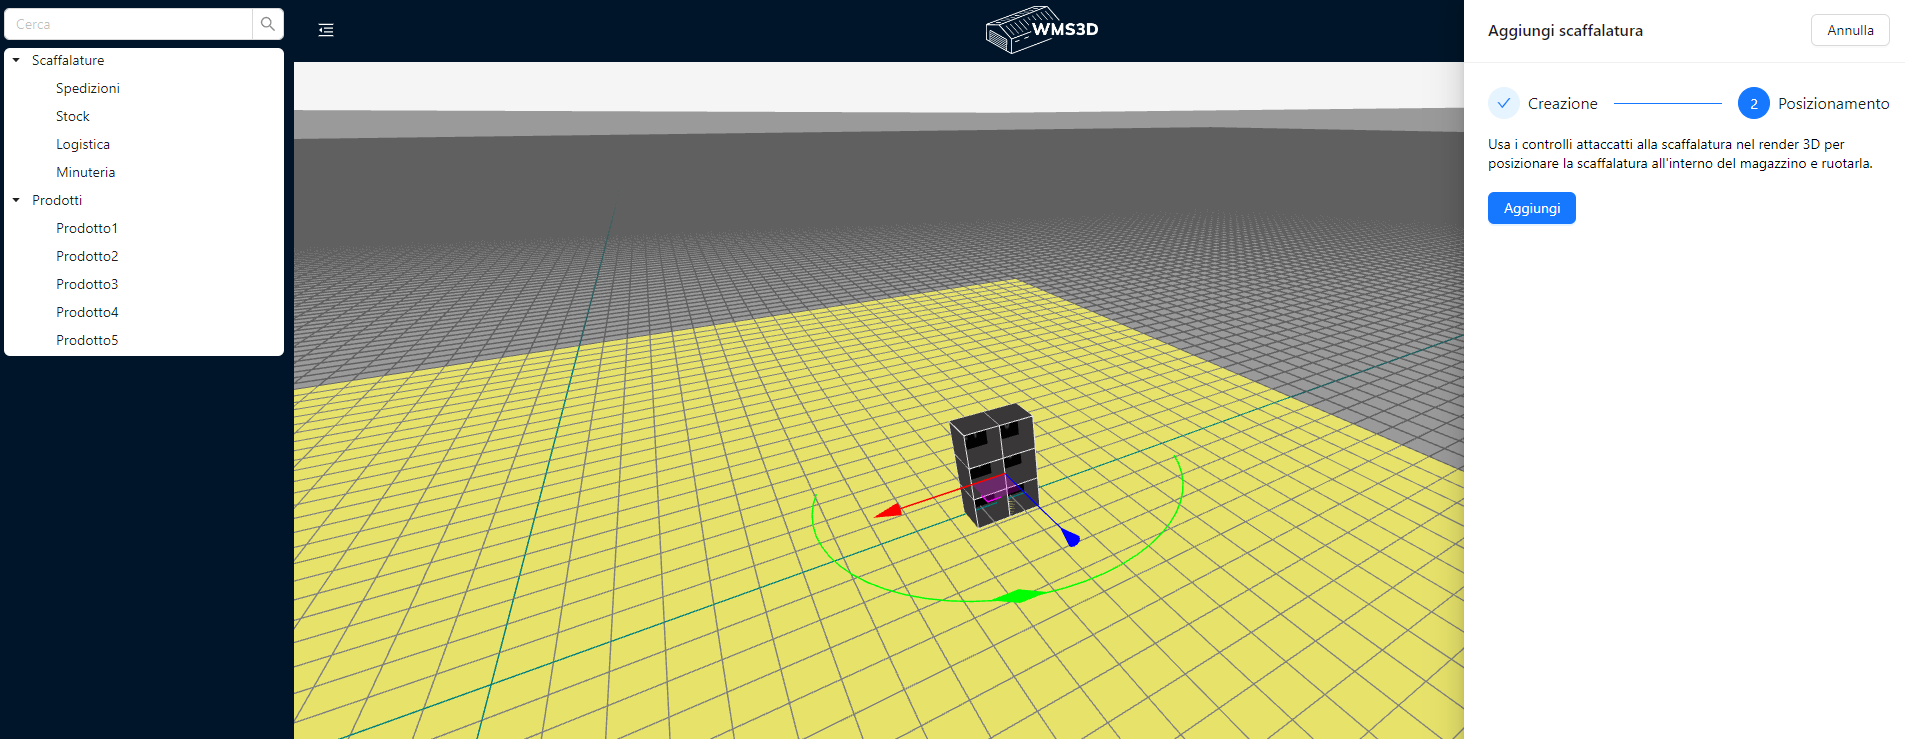
\includegraphics[width=0.8\textwidth]{images/posizionamento.png}
                \caption{Posizionamento scaffalatura}
            \end{figure}

            \noindent Una volta scelto il punto di posizionamento della scaffalatura completare il processo andando a confermare l'operazione con l'apposito tasto ``Aggiungi''. 
            In caso di posizione non conforme, i.e. non completamente interna al magazzino o intersecata ad altre scaffalatura, si visualizza il seguente errore. 
             \begin{figure}[H]
                \centering
                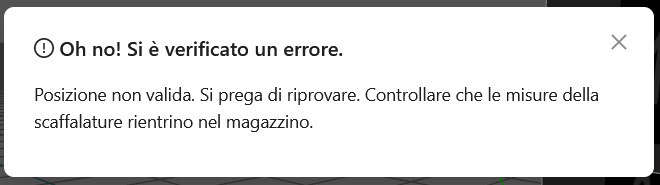
\includegraphics[width=0.5\textwidth]{images/errore_posizionamento.png}
                \caption{Errore posizionamento scaffalatura}
            \end{figure}
            \noindent Una volta chiusa la finestra sarà possibile riposizionare la scaffalatura. Nel caso non si trovi una posizione adatta è possibile annullare la creazione attraverso il pulsante ``Annulla'' posto sopra al modulo.


        \subsubsection{Modifica scaffalatura}\label{sec:scaffalature:modifica}
            Per modificare una scaffalatura esistente sarà sufficiente selezionare la scaffalatura desiderata (dal render 3D o dalla libreria) e premere il pulsante relativo all'operazione di interesse presente all'interno della Card. Le operazioni possibili sono l'eliminazione e la modifica.

            \bigskip
            \noindent L'\textbf{eliminazione} andrà ovviamente a rimuovere il componente sia dalla libreria che dal render 3D. 
            
            \noindent Il pulsante di eliminazione è indicato nell'immagine seguente.
            \begin{figure}[H]
                \centering
                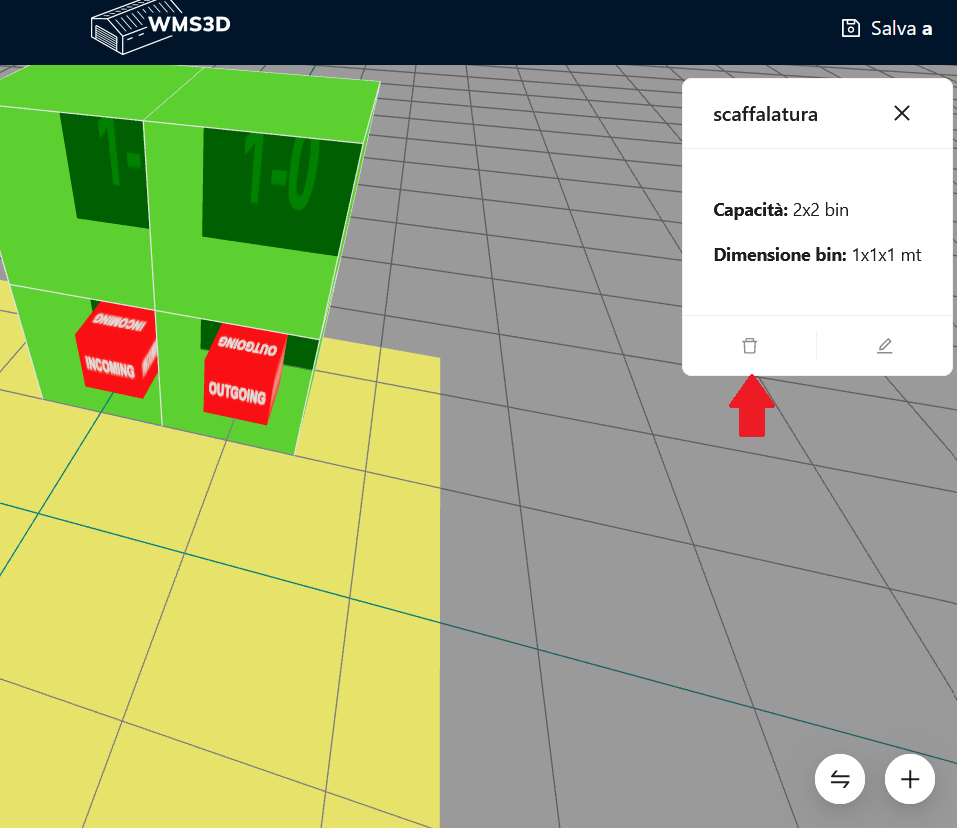
\includegraphics[width=0.5\textwidth]{images/pulsante_elimina_scaff.png}
                \caption{Card della scaffalatura - Pulsante eliminazione scaffalatura}
            \end{figure}

            \bigskip
            \noindent Con la \textbf{modifica}, invece, si entrerà nello stesso processo visto in precedenza con l'\hyperref[sec:scaffalature:aggiunta]{aggiunta scaffalatura} 
            e il \hyperref[sec:scaffalature:posizionamento]{posizionamento}. 
            Sarà quindi possibile cambiare nuovamente tutte le caratteristiche della scaffalatura e/o cambiarne la posizione nel render. 
            
            \noindent Il pulsante di modifica è indicato nell'immagine seguente.
            \begin{figure}[H]
                \centering
                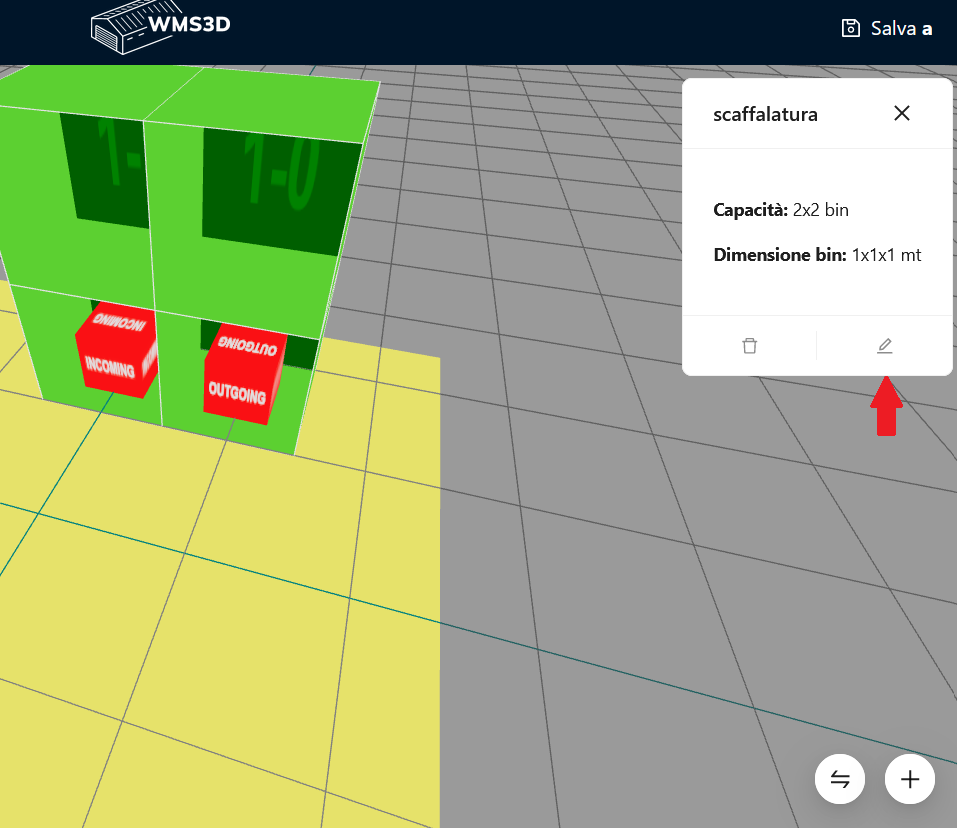
\includegraphics[width=0.5\textwidth]{images/pulsante_modifica_scaff.png}
                \caption{Card della scaffalatura - Pulsante modifica scaffalatura}
            \end{figure}

            \bigskip
            In entrambi i casi, è importante considerare la presenza di prodotti negli scaffali. Il sistema, infatti, impedisce la rimozione di scaffalature e bin in cui sono posizionati dei prodotti, mostrando un errore. Ad esempio, in caso di riduzione della capacità della scaffalatura con prodotti posizionati, viene visualizzato un errore del tipo:\\
            \begin{figure}[h!]
                \centering
                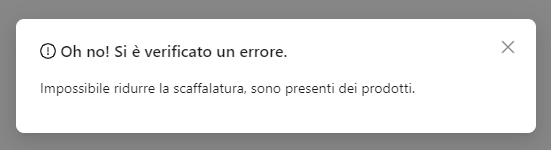
\includegraphics[width=0.5\textwidth]{images/errore_modifica.png}
                \caption{Errore modifica scaffalatura}
            \end{figure}

    \newpage            
    \subsection{Prodotti}\label{sec:prodotti}
    In questa sezione si riportano tutte le funzionalità disponibili per gestire i prodotti dal magazzino.
        \subsubsection{Aggiunta prodotto}\label{sec:prodotti:aggiunta}
        Per poter aggiungere una nuovo prodotto è necessario premere il tasto "+" presente nell'angolo in basso a destra del render 3D.\\
        \begin{figure}[h!]
            \centering
            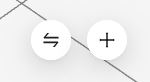
\includegraphics[width=0.3\textwidth]{images/aggiunta_spostamenti.png}
            \caption{Pulsante aggiunta componenti}
        \end{figure}
        
        \noindent Successivamente, per continuare, cliccare il tasto relativo all'aggiunta prodotto.\\
        \begin{figure}[h!]
            \centering
            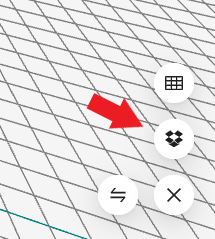
\includegraphics[width=0.3\textwidth]{images/aggiunta_prodotto.png}
            \caption{Pulsante aggiunta prodotto}
        \end{figure}

        \noindent Sarà quindi richiesto all'utente di creare il prodotto impostando i seguenti campi:
        \begin{itemize}
            \item Il \textbf{nome} che si intende dare al prodotto, che sarà univoco;
                \begin{itemize}
                        \item \textit{Formato accettato}: massimo 20 caratteri, scelti tra lettere (sia maiuscole che minuscole), numeri e "\_".
                \end{itemize}
            \item Il \textbf{colore} da assegnare al prodotto.
        \end{itemize}
        
        \begin{figure}[H]
            \centering
            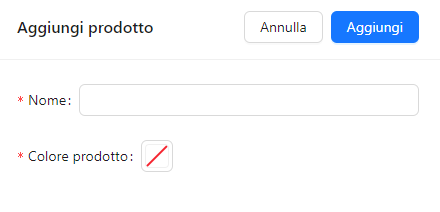
\includegraphics[width=0.6\textwidth]{images/creazione_prodotto.png}
            \caption{Form di aggiunta prodotto}
        \end{figure}

        \subsubsection{Posizionamento prodotto}\label{sec:prodotti:posizionamento}
        \noindent Una volta creato correttamente un prodotto si potrà posizionare il prodotto in un bin attraverso l'apposito pulsante.
        In particolare, dopo aver selezionato il prodotto dalla libreria e aperto dunque la Card del prodotto, sarà possibile cliccare sul pulsante di posizionamento (indicato nell'immagine sottostante) per poter andare a scegliere il bin di destinazione. 
        \begin{figure}[h!]
            \centering
            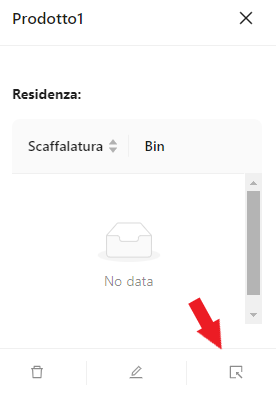
\includegraphics[width=0.3\textwidth]{images/tasto_posizionamento.png}
            \label{riposizionamento}
            \caption{Pulsante di posizionamento del prodotto}
        \end{figure}
        
        \noindent Si aprirà quindi la procedura guidata per andare ad identificare precisamente il bin di destinazione indicando, in ordine di presentazione:
        \begin{itemize}
            \item la \textbf{scaffalatura};
            \item il \textbf{ripiano} della scaffalatura;
            \item la \textbf{colonna} della scaffalatura.
        \end{itemize}
        \begin{figure}[H]
            \centering
            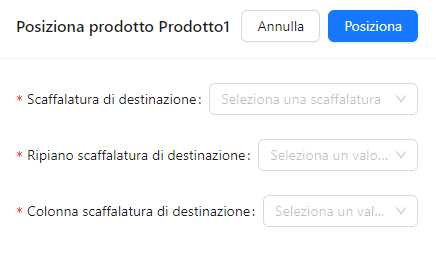
\includegraphics[width=0.4\textwidth]{images/scelta_posizione_prodotto.png}
            \label{destinazione_prodotto}
            \caption{Form di posizionamento del prodotto}
        \end{figure}
        
        \noindent Anche in questo caso si deve prestare attenzione in quanto i bin già occupati non possono ovviamente essere la destinazione di un secondo prodotto. 
        Tale tentativo segnalerebbe il seguente errore.\\
        \begin{figure}[H]
            \centering
            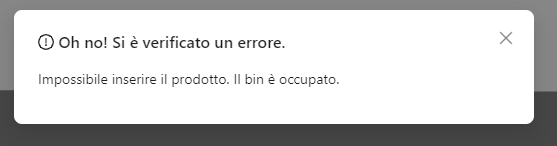
\includegraphics[width=0.5\textwidth]{images/bin_occupato.png}
            \caption{Errore: bin già occupato}
        \end{figure}
        
        \noindent Si noti che è possibile posizionare il prodotto in più bin, ripetendo il processo sopra descritto. I bin in cui è posizionato il prodotto verranno poi visualizzati tutti nella Card stessa del prodotto. 
    \newpage

    \subsubsection{Modifica prodotto}\label{sec:prodotti:modifica}
        \paragraph{Modifica del prodotto in tutte le sue copie}
        Per modificare un prodotto esistente sarà sufficiente selezionarlo dalla libreria e premere il pulsante relativo all'operazione di interesse presente 
        all'interno della Card del prodotto aperta attraverso la selezione. Le operazioni possibili sono l'eliminazione e la modifica.  

        \bigskip
        L'\textbf{eliminazione} andrà ovviamente a rimuoverlo dalla libreria e nel render 3D verranno rimosse tutte le sue copie (se presenti).
        
        \noindent Il pulsante di eliminazione è indicato nell'immagine seguente.
        \begin{figure}[H]
            \centering
            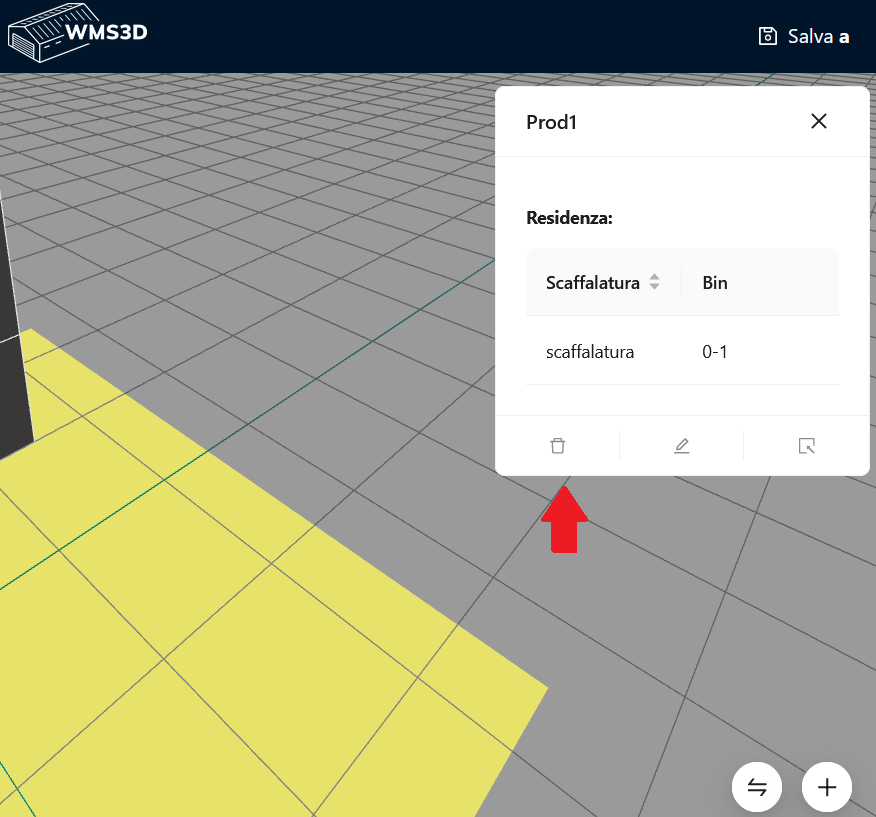
\includegraphics[width=0.5\textwidth]{images/pulsante_elimina_prod.png}
            \caption{Card del prodotto - Pulsante eliminazione prodotto}
        \end{figure}
        
        Con la \textbf{modifica} invece si entrerà nello stesso processo visto in precedenza con l'\hyperref[sec:prodotti:aggiunta]{aggiunta prodotto}. 
        Sarà quindi possibile cambiare nuovamente il nome e il colore del prodotto scelto. 
        
        \noindent Il pulsante di modifica è indicato nell'immagine seguente.
        \begin{figure}[H]
            \centering
            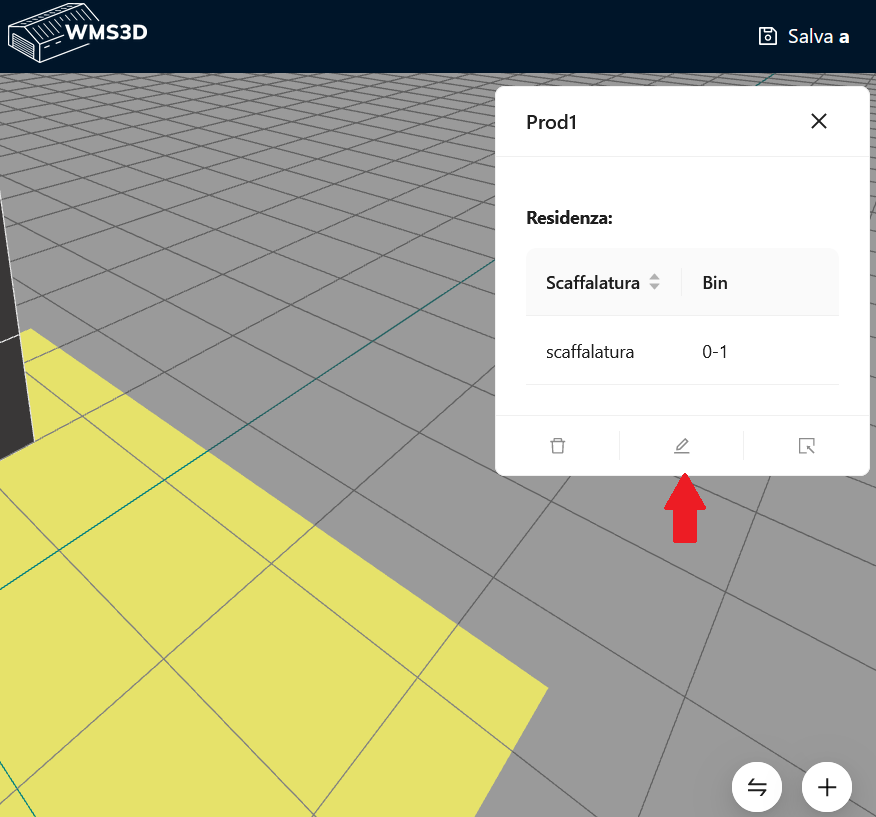
\includegraphics[width=0.5\textwidth]{images/pulsante_modifica_prod.png}
            \caption{Card del prodotto - Pulsante modifica prodotto}
        \end{figure}

        \paragraph{Modifica di un singolo prodotto posizionato}
        È possibile modificare alcune proprietà per singole copie del prodotto, posizionate in uno specifico bin. In particolare, si seleziona il bin (o attraverso render 3D o attraverso la Card del prodotto) e dalla Card del bin, così aperta, si potrà premere il pulsante relativo all'operazione di interesse. Le operazioni possibili sono l'eliminazione e la richiesta di movimentazione. Si noti che, ovviamente, queste operazioni saranno possibili soltanto se il bin selezionato contiene un prodotto al suo interno. Altrimenti verrà visualizzato un messaggio di errore simile al seguente (visualizzato nel caso di operazione di eliminazione).
        \begin{figure}[H]
            \centering
            
\includegraphics[width=0.4\textwidth]{images/errore_bin_vuoto.png}
            \caption{Errore operazioni su bin vuoto}
        \end{figure}
        
        
        \bigskip
        \noindent L'\textbf{eliminazione} andrà a rimuovere la copia del prodotto dalla lista nella Card del prodotto e nel render 3D verrà rimosso il prodotto dal bin selezionato. Lo stato del bin verrà dunque aggiornato di conseguenza.
        
        \noindent Il pulsante di eliminazione è indicato nell'immagine seguente.
        \begin{figure}[H]
            \centering
            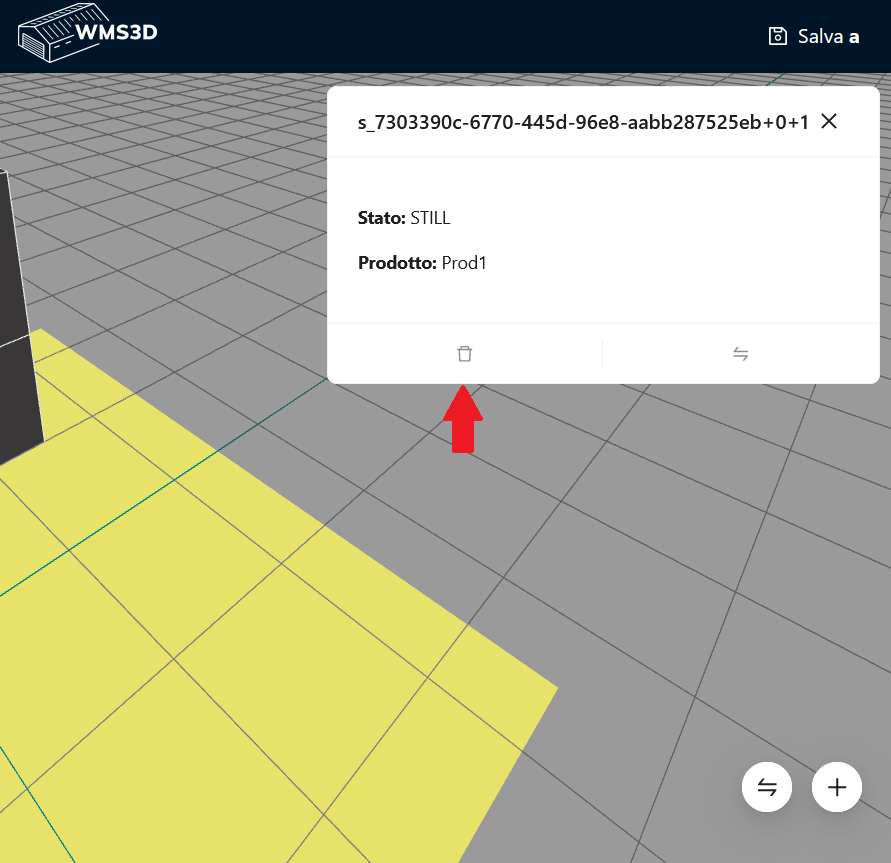
\includegraphics[width=0.5\textwidth]{images/pulsante_elimina_prod_bin.png}
            \caption{Card del bin - Pulsante modifica prodotto nel bin}
        \end{figure}
        
        \bigskip
        \noindent Tramite la \textbf{richiesta di movimentazione}, invece, si entrerà nello stesso processo visto in precedenza con la \hyperref[destinazione_prodotto]{scelta della destinazione}. Una volta selezionata correttamente la destinazione del prodotto il sistema andrà ad occupare il bin di arrivo creando un duplicato del prodotto in fase di spostamento. Avremo quindi un bin marchiato ``incoming'' e un bin marchiato ``outcoming'', entrambi visibili dalla Card del prodotto.
        
        \noindent Il pulsante di richiesta di movimentazione è indicato nell'immagine seguente.
        \begin{figure}[H]
                \centering
                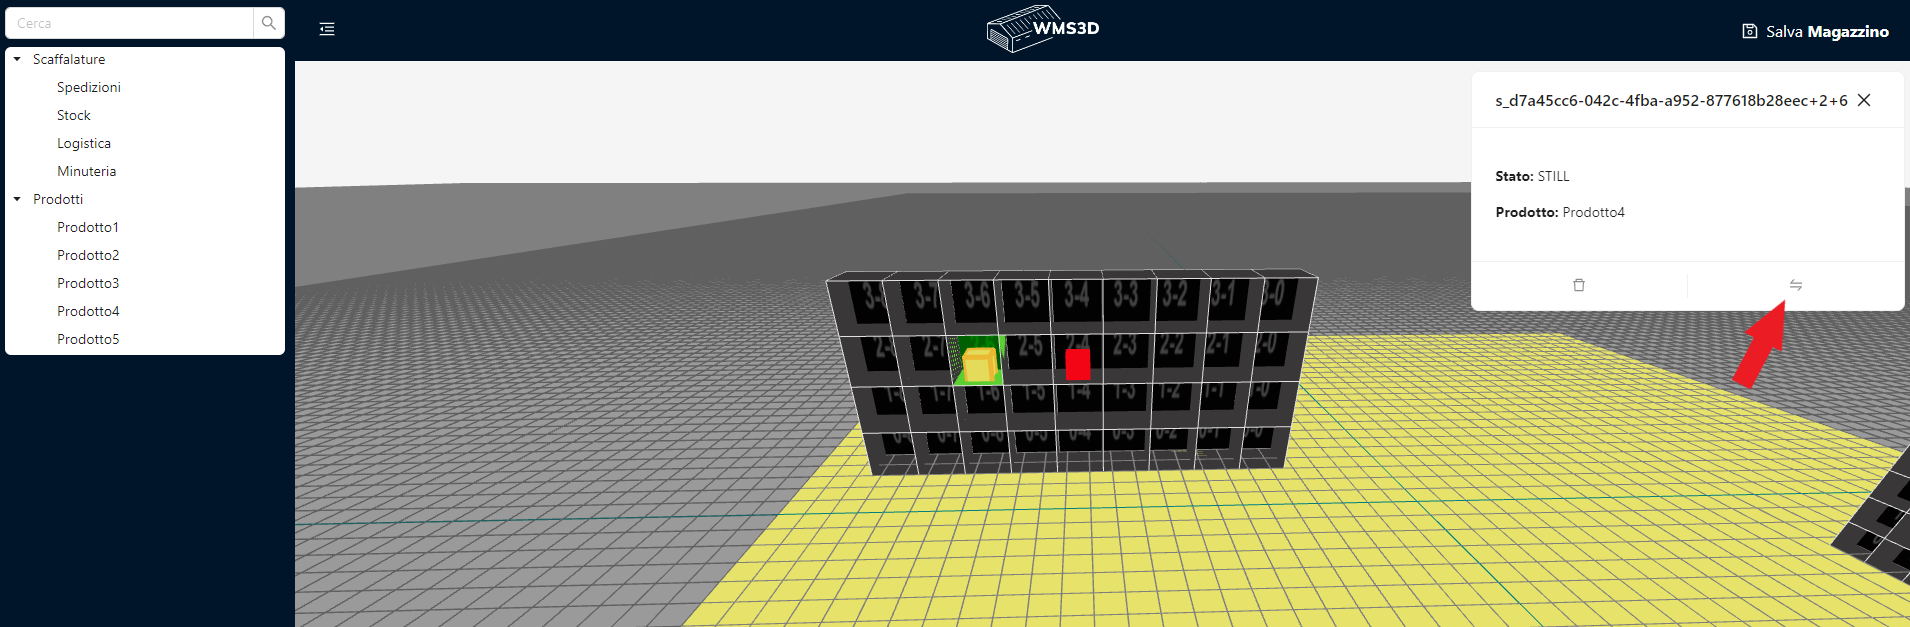
\includegraphics[width=1.0\textwidth]{images/movimentazione.png}
                \caption{Card del bin - Pulsante di richiesta di movimentazione del prodotto}
        \end{figure}
        
    \subsubsection{Lista movimenti} \label{sec:movimento:lista}
        È possibile consultare la lista dei prodotti attualmente in fase di spostamento selezionando l'apposito bottone in basso a destra nella sezione 3D.
        \begin{figure}[h!]
            \centering
            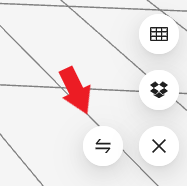
\includegraphics[width=0.2\textwidth]{images/pulsante_lista.png}
            \caption{Pulsante lista movimenti}
        \end{figure}\\
        \noindent Azionandolo si potrà accedere alla lista delle movimentazioni di prodotti ancora pendenti.
        Per ogni richiesta pendente sono riportati:
        \begin{itemize}
            \item Un \textbf{codice univoco della richiesta};
            \item La \textbf{scaffalatura, il ripiano e la colonna di origine}, in cui il prodotto si trova attualmente;
            \item La \textbf{scaffalatura, il ripiano e la colonna di destinazione}, verso cui il prodotto deve essere movimentato.
        \end{itemize}
        
        \begin{figure}[H]
            \centering
            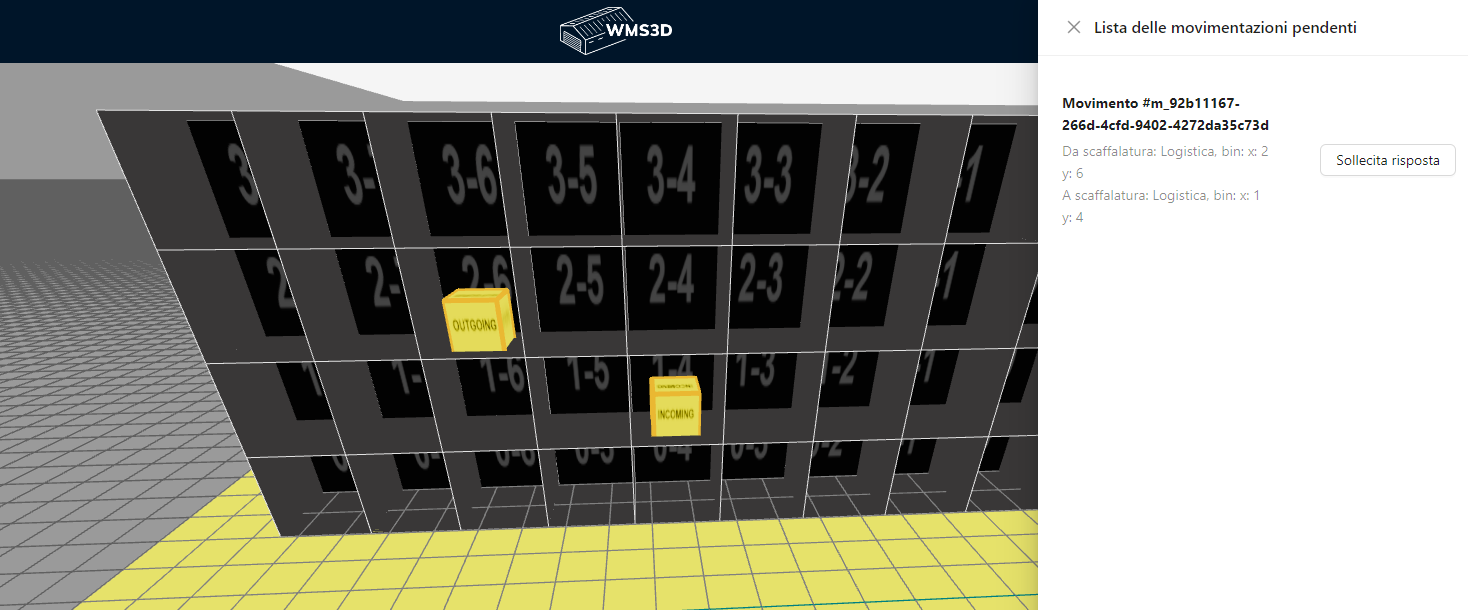
\includegraphics[width=1.0\textwidth]{images/lista_movimenti.png}
            \caption{Lista movimenti}
        \end{figure}
        Inoltre l'utente, attraverso il pulsante ``Sollecita risposta'' potrà richiedere il completamento di una singola richiesta di spostamento.
        Al termine di tale processo, il componente duplicato (``outcoming'' in caso di rifiuto o ``incoming'' in caso di accettazione) verrà rimosso 
        dal render 3D e verranno aggiornati gli stati dei bin di conseguenza. Verrà rimosso anche la richiesta di movimentazione pendente dalla lista.\\
        \begin{figure}[H]
            \centering
            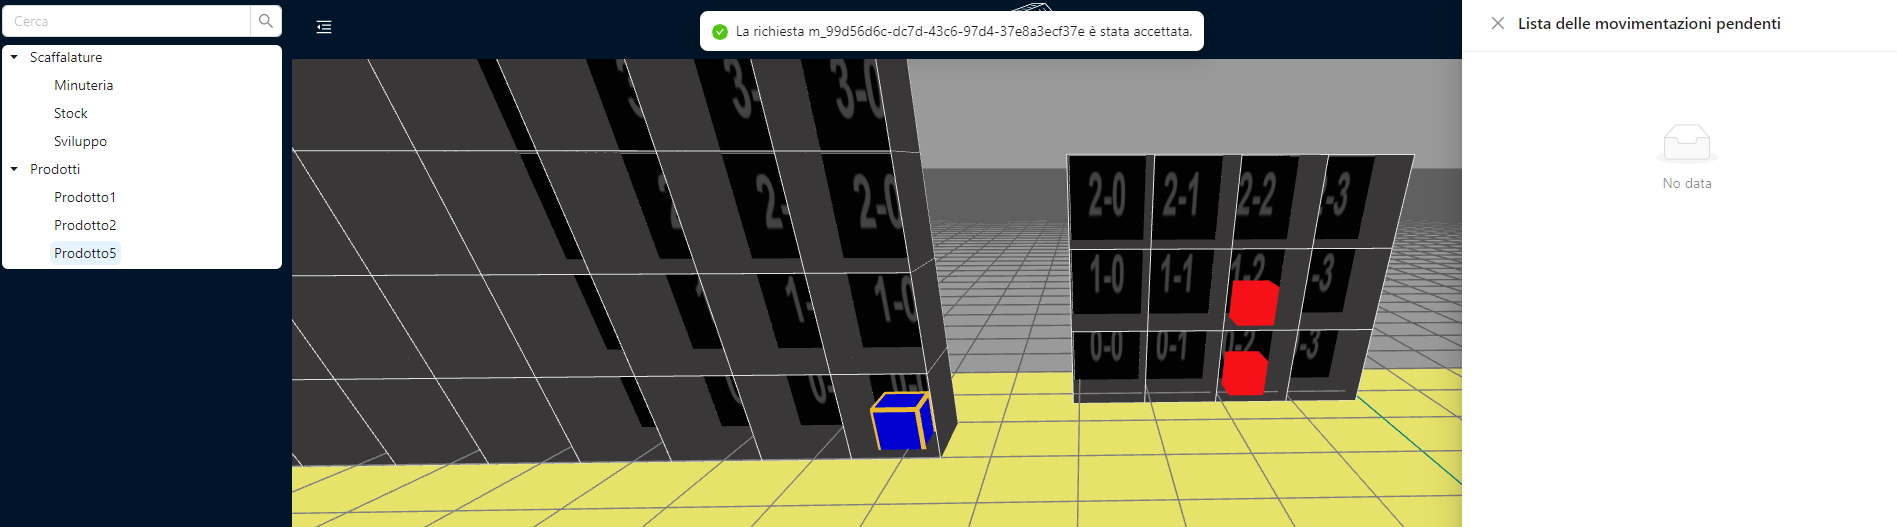
\includegraphics[width=1.0\textwidth]{images/ok_movimento.png}
            \caption{Esempio movimentazione approvata}
        \end{figure}

\newpage
\section{Glossario}
\subsection*{B}
\textbf{Bin}\\
Unità di dimensioni fisse con cui le scaffalature stesse sono misurate e suddivise. Scaffalature diverse possono avere bin di dimensioni diverse. Un bin può contenere al massimo un prodotto.

\subsection*{C}
\textbf{Card}\\
Componente grafica utilizzata per presentare informazioni in modo chiaro e compatto. Viene visualizzata come una finestra posta sopra al render 3D. Una Card contiene una collezione di informazioni correlate e delle azioni ad esse relative. Nello specifico sono realizzate tre diversi tipi di Card:
\begin{itemize}
    \item Card di una scaffalatura;
    \item Card di un prodotto;
    \item Card di un bin.
\end{itemize}

\subsection*{L}
\textbf{Libreria}\\
Con riferimento all’applicativo sviluppato, si intende un’area separata in cui visualizzare in maniera testuale i dati del magazzino, in particolare l'elenco di prodotti e delle scaffalature.

\subsection*{M}
\textbf{Modalità utente}\\
Modalità di esecuzione adatta agli utenti meno esperti in materia. Si tratta di accedere all'applicativo attraverso un link web fornito.

\bigskip
\noindent \textbf{Modalità programmatore}\\
Modalità di esecuzione adatta agli utenti più esperti. Consente di installare il progetto ed eseguirlo in locale.

\subsection*{P}
\textbf{Prodotto}\\
Si intende una categoria di prodotti. Possono essere allocati più prodotti di questa categoria all'interno del magazzino o può non esserne allocato nessuno. Il singolo prodotto fisico è da intendersi come il prodotto interno ad un bin.

\subsection*{R}
\textbf{Repository}\\
Archivio digitale centralizzato che contiene tutti i dati di progetto, inclusi codice e documentazione.

\subsection*{W}
\textbf{Warehouse Management System}\\
Applicazione software progettata per monitorare e ottimizzare le operazioni di stoccaggio e movimentazione delle merci all'interno di un magazzino. 

\newpage
%%%%%%%%%%%%%%%%%%%%%%%%%%%%%%%%%%%
% RIFERIMENTI ESTERNI
%%%%%%%%%%%%%%%%%%%%%%%%%%%%%%%%%%%

\section{Riferimenti esterni}\label{sec:riferimenti_esterni}
Per ulteriori chiarimenti sugli argomenti discussi nel documento, si possono consultare i seguenti link esterni:
\begin{itemize}
    \item Pagina di installazione al software \textbf{Node.js}:\\
    \url{https://nodejs.org/en/} \textcolor{gray}{\textit{(ultimo accesso 08-05-24)}}
\end{itemize}